\subsection{Adapter}
\subsubsection{Định nghĩa}
Adapter là một Structural Pattern cung cấp cho bạn thiết kế có thể phối hợp hai đối tượng với lớp cha kế thừa interface không tương thích nhau.
\subsubsection{Cách sử dụng}
Bạn nên sử dụng Adapter trong các trường hợp sau:
\begin{itemize}
    \item Khi bạn muốn kết nối hai lớp hoặc hệ thống không tương thích với nhau về giao diện.
    \item Khi bạn muốn tái sử dụng lại một lớp đã tồn tại trong một hệ thống mới mà không cần chỉnh sửa lớp đó.
\end{itemize}
\subsubsection{Cấu trúc}
\begin{itemize}
    \item ImageViewer có vai trò như adapter để chuyển đổi sang các dạng cần thiết để hiển thị.
\end{itemize}
\begin{center}
    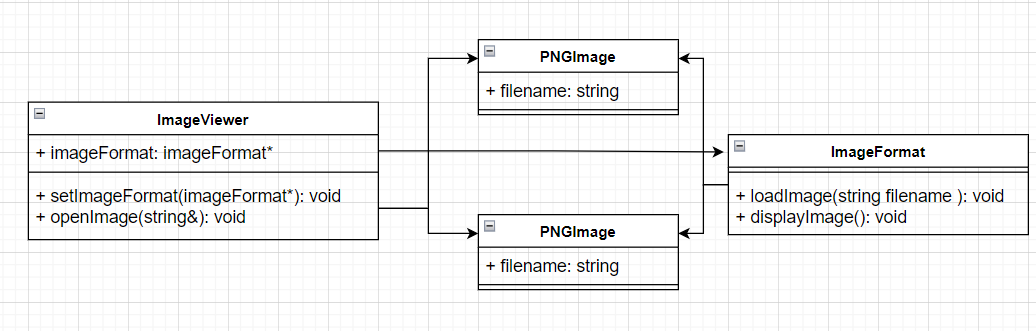
\includegraphics[scale=0.75]{image/structural/adapter.png}
\end{center}
Các thành phần chính:
\begin{itemize}
    \item Một class mô tả một giao thức mà các lớp khải phải tuân theo để hoạt động.
    \item Một Adapter để chuyển đối cách hoạt động của các hàm.
    \item Một class Service để thực hiện các hành vi cần thiết.
\end{itemize}
\subsubsection{Ưu điểm và Nhược điểm}
Ta có các ưu và nhược điểm dễ thấy sau:\\\\
Ưu điểm:
\begin{itemize}
    \item Adapter giúp kết nối các lớp hoặc hệ thống không tương thích với nhau về giao diện và cho phép chúng làm việc cùng nhau.
    \item Adapter cho phép tái sử dụng lại các lớp đã tồn tại và mở rộng chức năng của chúng mà không cần thay đổi lớp gốc.
\end{itemize}
Nhược điểm:
\begin{itemize}
    \item Adapter không thể giải quyết các trường hợp tương thích mạnh hơn, trong đó sự khác biệt giữa các giao diện là quá lớn để có thể chuyển đổi trực tiếp.
\end{itemize}
\subsubsection{Code Example}
\begin{itemize}
    \item Ta có 2 loại hình ảnh là Png và Jpeg.
    \item Các loại hình ảnh có 2 phương thức là tải hình ảnh lên và hiển thị hình ảnh.
    \item Ta có giao diện người xem sẽ chứa thuộc tính format của loại hình ảnh hoạt động như một adapter để chuyển qua lại loại hình ảnh nhờ hàm setImageFormat().
\end{itemize}
\begin{lstlisting}
#include <iostream>
#include <string>

class ImageFormat {
public:
    virtual void loadImage(const std::string& filename) = 0;
    virtual void displayImage() = 0;
};

class PNGImage : public ImageFormat {
private:
    std::string filename;

public:
    void loadImage(const std::string& filename) override {
        this->filename = filename;
        std::cout << "Loading PNG image: " << filename << std::endl;
    }

    void displayImage() override {
        std::cout << "Displaying PNG image: " << filename << std::endl;
    }
};

class JPEGImage : public ImageFormat {
private:
    std::string filename;

public:
    void loadImage(const std::string& filename) override {
        this->filename = filename;
        std::cout << "Loading JPEG image: " << filename << std::endl;
    }

    void displayImage() override {
        std::cout << "Displaying JPEG image: " << filename << std::endl;
    }
};

class ImageViewer {
private:
    ImageFormat* imageFormat;

public:
    void setImageFormat(ImageFormat* format) {
        imageFormat = format;
    }

    void openImage(const std::string& filename) {
        imageFormat->loadImage(filename);
        imageFormat->displayImage();
    }
};

int main() {
    ImageViewer viewer;

    viewer.setImageFormat(new PNGImage());
    viewer.openImage("image.png");

    viewer.setImageFormat(new JPEGImage());
    viewer.openImage("image.jpg");

    return 0;
}

\end{lstlisting}
Ở hàm main, ta gọi một giao diện người dùng và lần lượt chỉnh giao diện đó thành loại hình ảnh Png và Jpeg và mở lần lượt xen kẻ.\\
\newline
\textbf{Kết quả:}
\begin{lstlisting}
Loading PNG image: image.png
Displaying PNG image: image.png
Loading JPEG image: image.jpg
Displaying JPEG image: image.jpg
\end{lstlisting}
\subsubsection{Các Pattern liên quan}
\begin{itemize}
    \item Bride: có cấu trúc khá giống với Adapter nhưng khác nhau về mặt sử dụng.
    \item Decorator: hoặc ta có thể tăng cường class cần chuyển đối bằng decorator.
    \item Proxy: hoặc có thể tạo một Proxy class tương ứng với sản phẩm để nó tương tác với người dùng và chuyển đối qua Proxy khác trước khi truy cập trực tiếp vào đối tượng chính.
\end{itemize}